\documentclass[a4paper]{report}
\usepackage{makeidx}
\usepackage{graphicx}
%\graphicspath{ {./imagenes/} }
\usepackage{multicol}
\usepackage{float}
\usepackage{listings}
\usepackage{color}
\usepackage{ifthen}
\usepackage[table]{xcolor}
\usepackage{textcomp}
\usepackage{alltt}
\usepackage{ifpdf}
\usepackage{amsmath}
\ifpdf
\usepackage[pdftex,
            pagebackref=true,
            colorlinks=true,
            linkcolor=blue,
            unicode
           ]{hyperref}
\else
\usepackage[ps2pdf,
            pagebackref=true,
            colorlinks=true,
            linkcolor=blue,
            unicode
           ]{hyperref}
\usepackage{pspicture}
\fi
\usepackage[utf8]{inputenc}
\usepackage{mathptmx}
\usepackage[scaled=1]{helvet}
\usepackage{courier}
\usepackage{sectsty}
\usepackage[titles]{tocloft}
\usepackage{doxygen}
\usepackage[spanish]{babel}
\lstset{language=Python,inputencoding=utf8,basicstyle=\footnotesize,breaklines=true,breakatwhitespace=true,tabsize=8,numbers=left }
\makeindex
\setcounter{tocdepth}{3}
\renewcommand{\footrulewidth}{0.4pt}
\renewcommand{\familydefault}{\sfdefault}
\begin{document}
\hypersetup{pageanchor=false}
\begin{titlepage}
\vspace*{7cm}
\begin{center}
{\Huge Manual de Referencia}\\
\vspace*{1cm}
{\Huge DIRe}\\
\vspace*{1cm}
{\LARGE Jesus Casado Gonzalez}\\
\vspace*{0.5cm}
{\LARGE Gustavo Plaza Roma}\\
\vspace*{0.5cm}
{\Large \today}\\
\end{center}
\end{titlepage}
%\clearemptydoublepage
\pagenumbering{roman}
\tableofcontents
%\clearemptydoublepage
\pagenumbering{arabic}
\hypersetup{pageanchor=true}
\chapter{Introducción}
	Este manual pretende describir el funcionamiento de la aplicación \textit{DIRe}, esta aplicación tiene como finalidad realizar los cálculos necesarios para el diseño de reactores ideales.
	
	Esta aplicación se ha desarrollado usando Python 3, la interfaz gráfica se ha creado con el programa \textit{Qt Designer} y se ha transformado a Python para que sea compatible con la librería \textit{PySide 1.2.4}. 
	
	Pues que la librería \textit{PySide 1.2.4} no es compatible con Python 3.5, se usará Python 3.4. Es posible usar la versión 3.5 si se tiene instalado la \textit{PySide 2}.
	
	Para el correcto funcionamiento de la aplicación es necesario tener los siguientes módulos instalados:
	\begin{itemize}
		\item Pyqtgraph para poder visualizar gráficas dentro de la aplicación Qt.
		\item Matplotlib para poder visualizar y exportar los resultado de los cálculos.
		\item Scipy permite realizar las distintas operaciones matemáticas.
		\item Numpy proporciona las clases necesarias para operar con vectores.
	\end{itemize}
	
	%\newpage
	
	La aplicación está dividida en distintas ventanas según se verá a lo largo de este documento.
	
\section{Ventana principal y ventana de selección}
	La primera ventana que aparece al ejecutar la aplicación se puede ver en la Figura \ref{vent_prin}. Desde esta ventana se pueden realizar las siguientes acciones:
	\begin{itemize}
		\item Acceder a la ventana de selección del reactor.
		\item Salir de la aplicación.
		\item Visualizar la guía de usuario de la aplicación, en esta guía se muestran las ecuaciones usadas para el diseño de los reactores y los parámetros necesarios. Ver Figura \ref{vent_ayuda}
	\end{itemize}

	\begin{figure}[!h]
		\centering
		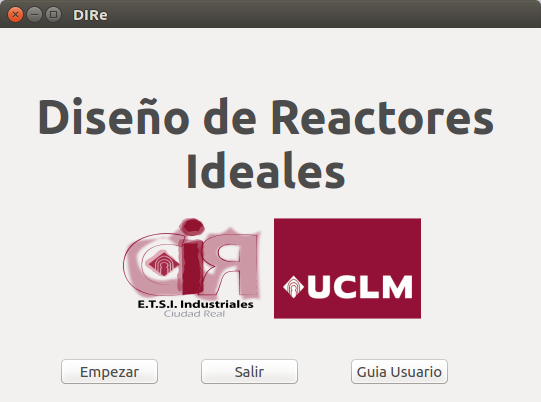
\includegraphics[width=0.8\textwidth]{./imagenes/DIRe_051.png}
		\label{vent_prin}
		\caption{Ventana Principal}
	\end{figure}
	
	\begin{figure}[!h]
		\centering
		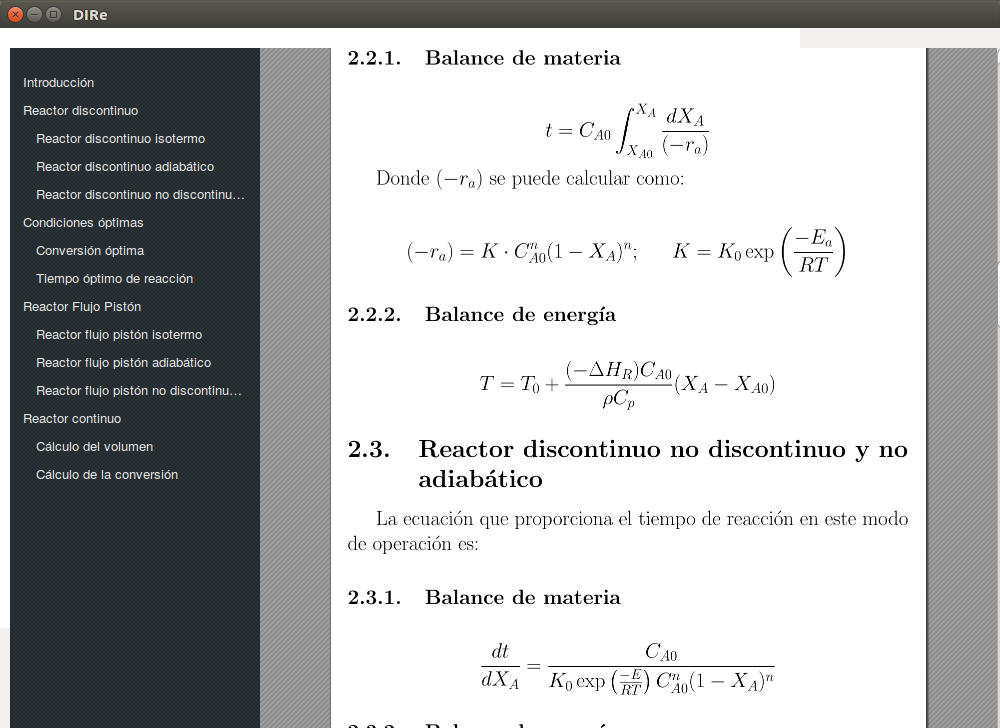
\includegraphics[width=0.8\textwidth]{./imagenes/DIRe_050.png}
		\label{vent_ayuda}
		\caption{Ventana de ayuda}
	\end{figure}

	En la ventana de selección se muestran botones que permiten seleccionar entre los distintos tipos de reactores. Los reactores que se pueden calcular son:
	
	\begin{itemize}
		\item Reactores discontinuos, dentro de este tipo se divide en isotermos, adiabáticos y otro tipo que no es ni adiabático ni isotermo.
		\item Reactores continuos (flujo pistón), dentro de este tipo se divide en isotermos, adiabáticos y otro tipo que no es ni adiabático ni isotermo.
		\item Reactores de lecho fijo.
	\end{itemize}

	En la Figura \ref{vent_seleccion} se puede ver la ventana de selección.
	
	\begin{figure}[!h]
		\centering
		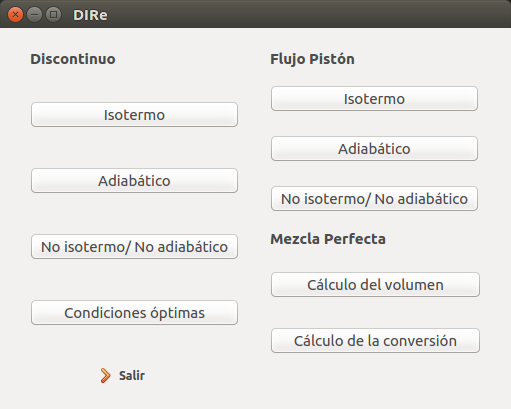
\includegraphics[width=0.8\textwidth]{./imagenes/DIRe_060.png}
		\label{vent_seleccion}
		\caption{Ventana de selección}
	\end{figure}


\chapter{Rector Discontinuo}
	Son aquellos que trabajan por cargas, es decir se introduce una alimentación, y se espera un tiempo dado, que viene determinado por la cinética de la reacción, tras el cual se saca el producto.
	
	\section{Reactor discontinuo isotermo}
	A partir del balance de materia se obtiene la ecuación que proporciona el tiempo de reacción a partir de la velocidad de reacción en este modo de operación es:
	
	\begin{equation*}
	t = C_{A0}\int_{X_{A0}}^{X_A}\frac{dX_A}{(-r_a)}
	\end{equation*}
	
	Donde $(-r_a)$ se puede calcular como:
	
	\begin{equation*}
	(-r_a) = K \cdot C_{A0}^n (1-X_A)^n; ~~~~~ K = K_0\exp\left(\frac{-E_a}{RT}\right)
	\end{equation*}
	
	Según el orden de reacción el tiempo se podrá calcular como:
	
	\begin{itemize}
		\item Orden 0: $ t = \frac{C_{A0}}{K}(X_A-X_{A0})$
		\item Orden 1: $ t = \frac{1}{K}\ln\left(\frac{1-X_{A0}}{1-X_A}\right)$
		\item Orden 2: $ t = \frac{1}{KC_{A0}}\left(\frac{X_A}{1- X_A}\right)$
	\end{itemize}
	
	En la Figura \ref{dis_iso} se puede ver la pantalla para definir los parámetros del reactor que son: 
	\begin{itemize}
		\item Orden de reacción.
		\item Temperatura inicial [K].
		\item Concentración inicial [mol/l].
		\item Energía de activación [J/mol].
		\item Constante $k_0$.
		\item Conversión inicial y final.
	\end{itemize}
	\begin{figure}[!h]
		\centering
		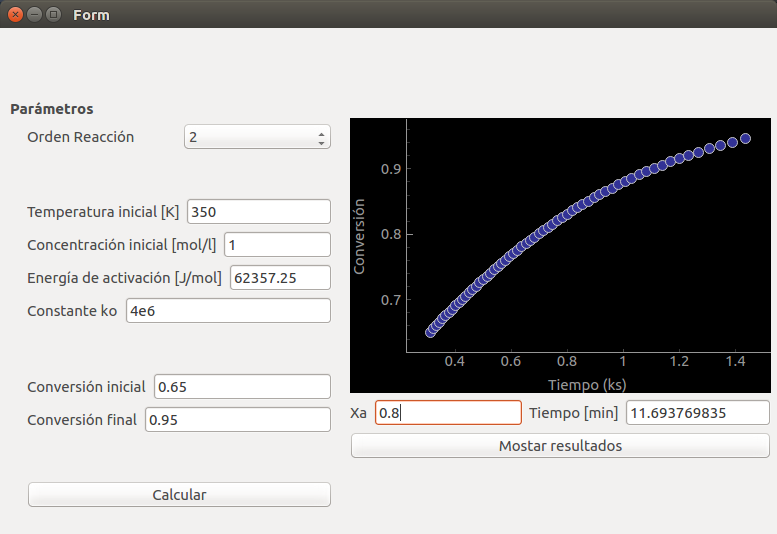
\includegraphics[width=0.9\textwidth]{./imagenes/reactor_discontinuo/Form_048.png}
		\label{dis_iso}
		\caption{Ventana de cálculo del reactor discontinuo e isotermo.}
	\end{figure}

	La aplicación tiene un cuadro de texto donde se puede introducir una conversión y automáticamente se rellena el campo que se encuentra al lado con el tiempo en  minutos que se tarda en alcanzar esa conversión. Todos los reactores cuentan también con esta característica.
	
	Todas las ventanas también cuentan con un botón que pone ``Mostrar resultados'' este botón genera una nueva ventana donde se puede ver la misma gráfica con un cursor para poder ver los datos de la curva. Esta ventana también permite guardar la gráfica. En la Figura \ref{dis_iso_graf} se puede ve la ventana generada con el botón ``Mostrar resultados''.
	
	\begin{figure}[!h]
		\centering
		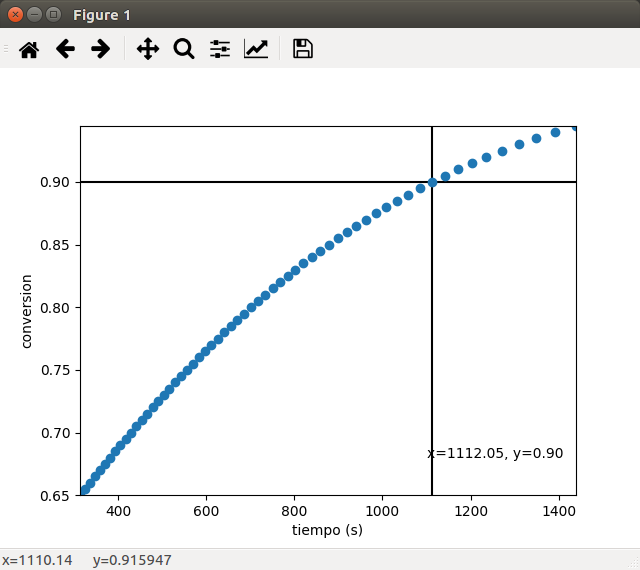
\includegraphics[width=0.9\textwidth]{./imagenes/reactor_discontinuo/iso_fig.png}
		\label{dis_iso_graf}
		\caption{Ventana con el resultado de un reactor isotermo.}
	\end{figure}
	
	\section{Reactor discontinuo adiabático}
	La ecuación que proporciona el tiempo de reacción en este modo de operación es:
	
	A partir del balance de materia se obtiene:
	\begin{equation*}
	t = C_{A0}\int_{X_{A0}}^{X_A}\frac{dX_A}{(-r_a)}
	\end{equation*}
	
	Donde $(-r_a)$ se puede calcular como:
	
	\begin{equation*}
	(-r_a) = K \cdot C_{A0}^n (1-X_A)^n; ~~~~~ K = K_0\exp\left(\frac{-E_a}{RT}\right)
	\end{equation*}
	
	A partir del balance de energía se obtiene:
	\begin{equation*}
	T = T_0 + \frac{(-\Delta H_R)C_{A0}}{\rho C_p}(X_A-X_{A0})
	\end{equation*}
	
	Los parámetros necesarios para el diseño del reactor son:
	
	\begin{itemize}
		\item Orden de reacción.
		\item Temperatura inicial [K].
		\item Concentración inicial [mol/l].
		\item Energía de activación [J/mol].
		\item Constante $k_0$.
		\item Calor de reacción [J/mol].
		\item Peso molecular [g/mol].
		\item Calor específico [J/(kg·K)].
		\item Densidad de la mezcla [kg/m3].
		\item Tipo de reacción (exotérmica, endotérmica).
		\item Conversión inicial y final.
	\end{itemize}

	En la Figura \ref{dis_adi} se puede ver la ventana para el cálculo de un reactor discontinuo y adiabático.
	
	\begin{figure}[!h]
		\centering
		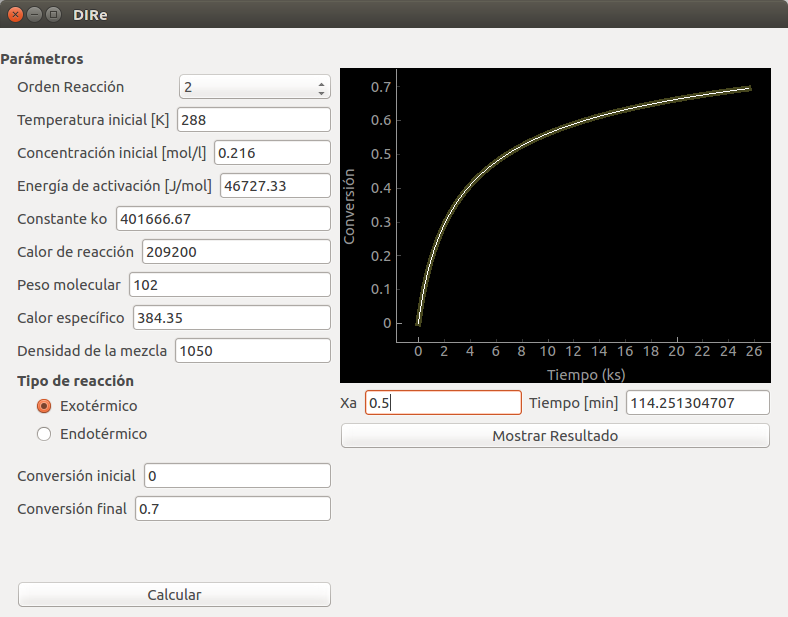
\includegraphics[width=0.9\textwidth]{./imagenes/reactor_discontinuo/adi.png}
		\label{dis_adi}
		\caption{Ventana de cálculo del reactor discontinuo y adiabático.}
	\end{figure}

	\section{Reactor discontinuo no discontinuo y no adiabático}
	La ecuación que proporciona el tiempo de reacción en este modo de operación es:
	
	A partir del balance de materia se obtiene:
	\begin{equation*}
	\frac{dt}{dX_A} = \frac{C_{A0}}{K_0 \exp\left(\frac{-E}{RT}\right) C_{A0}^n (1-X_A)^n}
	\end{equation*}
	
	A partir del balance de energía se obtiene:
	\begin{equation*}
	\frac{dT}{dX_A} = \frac{(-\Delta H_R)C_{A0}}{\rho C_p} + \frac{C_{A0}US(T_c-T)}{V\rho C_p K_0 \exp\left(\frac{-E_a}{RT}\right)C_{A0}^n(1-X_A)^n}
	\end{equation*}
	
	Los parámetros necesarios para el diseño del reactor son:
	
	\begin{itemize}
		\item Orden de reacción.
		\item Temperatura inicial [K].
		\item Concentración inicial [mol/l].
		\item Energía de activación [J/mol].
		\item Constante $k_0$.
		\item Calor de reacción [J/mol].
		\item Peso molecular [g/mol].
		\item Calor específico [J/(kg·K)].
		\item Densidad de la mezcla [kg/m3].
		\item Coeficiente de transmisión de calor [W/(m·K)].
		\item Área de transmisión de calor [m2].
		\item Volumen [m3]. 
		\item Tipo de reacción (exotérmica, endotérmica).
		\item Conversión inicial y final.
	\end{itemize}
	
	En la Figura \ref{dis_no_iso_no_adi} se puede ver la ventana para el cálculo de un reactor discontinuo que no es isotermo ni adiabático.
	\begin{figure}[!h]
		\centering
		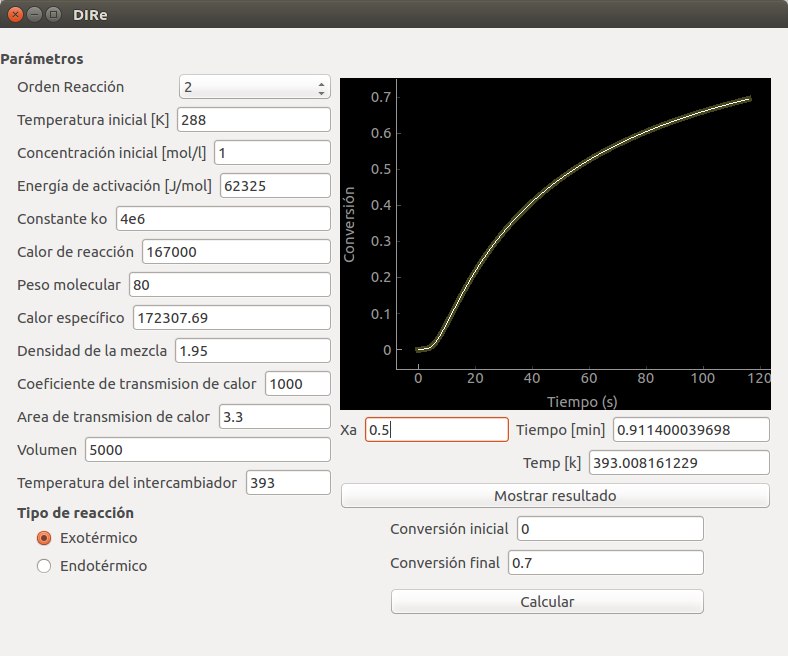
\includegraphics[width=0.9\textwidth]{./imagenes/reactor_discontinuo/no_iso_no_adi.png}
		\label{dis_no_iso_no_adi}
		\caption{Ventana de cálculo del reactor discontinuo que no es isotermo ni adiabático.}
	\end{figure}

	
	En este tipo de reactor cuando se pulsa el botón de ``Mostrar resultados'' se muestran dos gráficas, una de ellas muestra la conversión frente al tiempo y la otra la temperatura frente al tiempo. Ver Figura \ref{dis_no_iso_no_adi_fig}.
	
	\begin{figure}[!h]
		\centering
		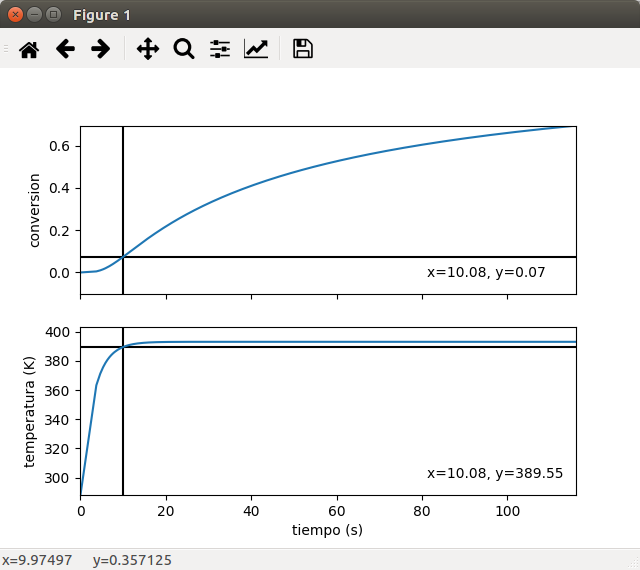
\includegraphics[width=0.8\textwidth]{./imagenes/reactor_discontinuo/no_iso_no_adi_fig.png}
		\label{dis_no_iso_no_adi_fig}
		\caption{Resultado del cálculo del reactor discontinuo que no es isotermo ni adiabático.}
	\end{figure}
\chapter{Condiciones óptimas}
	\section{Condiciones óptimas}
	Esta parte de la aplicación permite llevar a cabo la optimización de costes.
	
	
	Para calcular la conversión óptimas se usa la siguiente expresión:
	
	\begin{equation*}
		X_{A_{opt}} = 1- \frac{C_Ra}{(\Delta w) C_{A0}VK}
	\end{equation*}
	
	Para calcular el tiempo óptimo se usa la siguiente expresión:
	
	\begin{equation*}
		t_{opt} = \frac{1}{K}\ln \left(\frac{(\Delta w) C_{A0}VK}{C_Ra}\right)
	\end{equation*}
	
	Los parámetros necesarios para el cálculo de las condiciones óptimas son:
	
	\begin{itemize}
		\item Orden de reacción.
		\item Temperatura inicial [K].
		\item Concentración inicial [mol/l].
		\item Energía de activación [J/mol].
		\item Constante $k_0$.
		\item Volumen [m3].
		\item Coste de reacción [€/s]
		\item Valor aumentado por mol transformado [€].
	\end{itemize}
	
	En la Figura \ref{con_op} se puede ver la ventana para el cálculo de las condiciones
	óptimas para la reacción.

	\begin{figure}[!h]
		\centering
		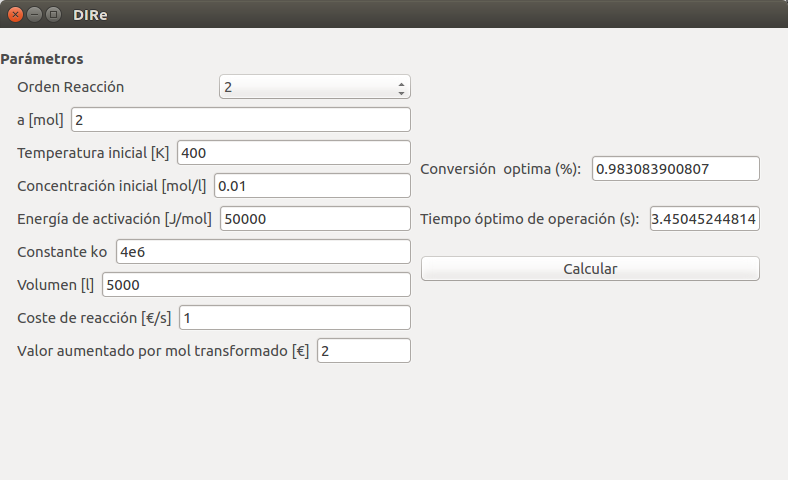
\includegraphics[width=0.9\textwidth]{./imagenes/reactor_discontinuo/con_op.png}
		\label{con_op}
		\caption{Ventana para el cálculo de las condiciones óptimas para la reacción.}
	\end{figure}

	

\chapter{Reactor Flujo Pistón}
	El reactor de flujo pistón trabaja en estado estacionario. Esto significa que las propiedades no varían con el tiempo.
	
	En el menú principal, encontramos tres botones dentro del apartado de reactores flujo pistón. Estos tres botones hacen referencia cada a uno a distintas condiciones en las que el reactor puede realizar su operación: reactor flujo pistón isotermo, reactor flujo pistón adiabático y reactor flujo pistón ni isotermo ni adiabático.
	
\section{Reactor flujo pistón isotermo}
Si seleccionamos el caso del reactor flujo pistón isotermo, nos aparece una ventana como la que se puede observar en la Figura \ref{fig:ventana_isotermo}.

\begin{figure}[h!]
	\begin{center}
		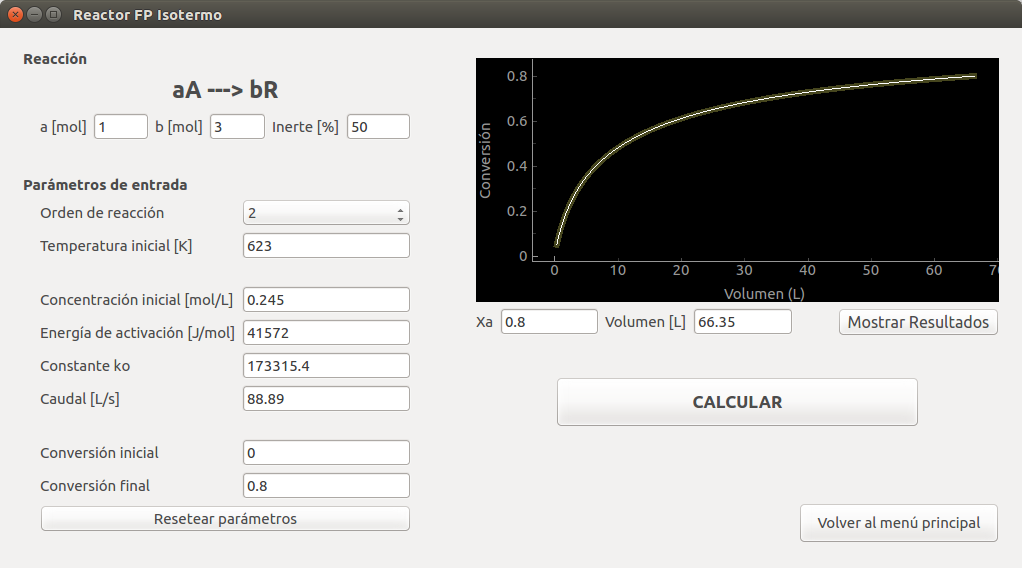
\includegraphics[width=0.85\textwidth]{./imagenes/reactor_fp/isotermo1.png}\caption{Ventana reactor FP isotermo}\label{fig:ventana_isotermo}
	\end{center}
\end{figure}

En la parte superior izquierda, el programa nos indica el tipo de reacción con la que vamos a trabajar y permite modificar el número de reactivos y productos, así como añadir el porcentaje deseado de inerte en la reacción. Una vez que hayamos establecido la reacción deseada, deberemos seleccionar el orden de reacción en el desplegable e introducir todos los parámetros de entrada indicados, prestando especial atención a las unidades en las que se indican que han de ser introducidos.

Cuando tengamos introducidos todos los datos que se indican, podremos obtener el resultado final pulsado sobre el botón \textbf{'CALCULAR'} situado en la parte derecha de la ventana. Inmediatamente después de pulsar sobre dicho botón el programa representará gráficamente el resultado en el gráfico de la parte derecha de la ventana, y se indicará el resultado obtenido, en función de nuestros parámetros de entrada, en las celdas situadas en la parte inferior del gráfico.

Otra de las opciones que pone a nuestra disposición este software es la de observar el gráfico en una ventana independiente ((Figura \ref{fig:ventana_graficas_iso})), pulsado sobre el botón \textbf{'Mostrar Resultados'}. En esta nueva ventana, no solo podremos ver el mismo gráfico descrito anteriormente, sino que además dispondremos de un cursor que nos permitirá ver el resultado en cada punto deseado (antes el resultado dado en las celdas inferiores al gráfico solo mostraba el resultado teniendo en cuenta los parámetros de entrada). En esta nueva ventana también se nos permite exportar el gráfico como una imagen.

\begin{figure}[h!]
	\begin{center}
		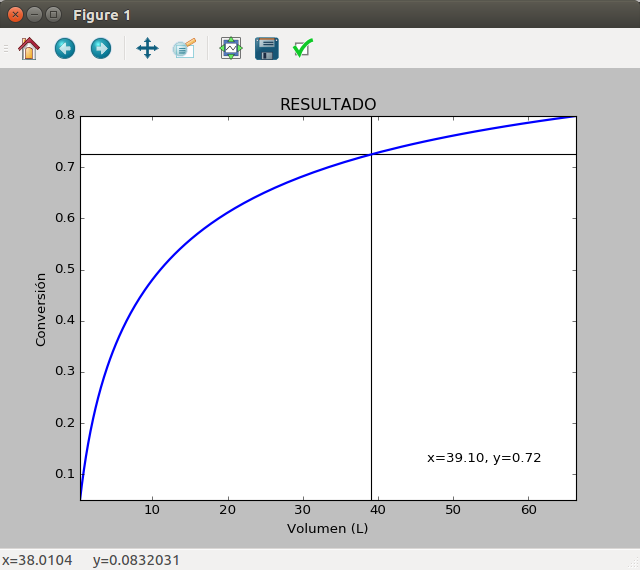
\includegraphics[width=0.85\textwidth]{./imagenes/reactor_fp/isotermo2.png}\caption{Ventana de resultados reactor FP isotermo}\label{fig:ventana_graficas_iso}
	\end{center}
\end{figure}

Finalmente, podemos realizar un borrado de todas las celdas, mediante el botón \textbf{'Resetear parámetros'}, para realizar un nuevo cálculo. Si no deseamos realizar más cálculos y queremos regresar al menú principal, podremos hacerlo pinchando sobre el botón mediante el botón \textbf{'Volver al menú principal'} de abajo a la derecha de la ventana.


\section{Reactor flujo pistón adiabático}
Seleccionando el reactor flujo pistón adiabático, se nos abrirá una ventana como la mostrada en la Figura \ref{fig:ventana_adiabatico}.

\begin{figure}[h!]
	\begin{center}
		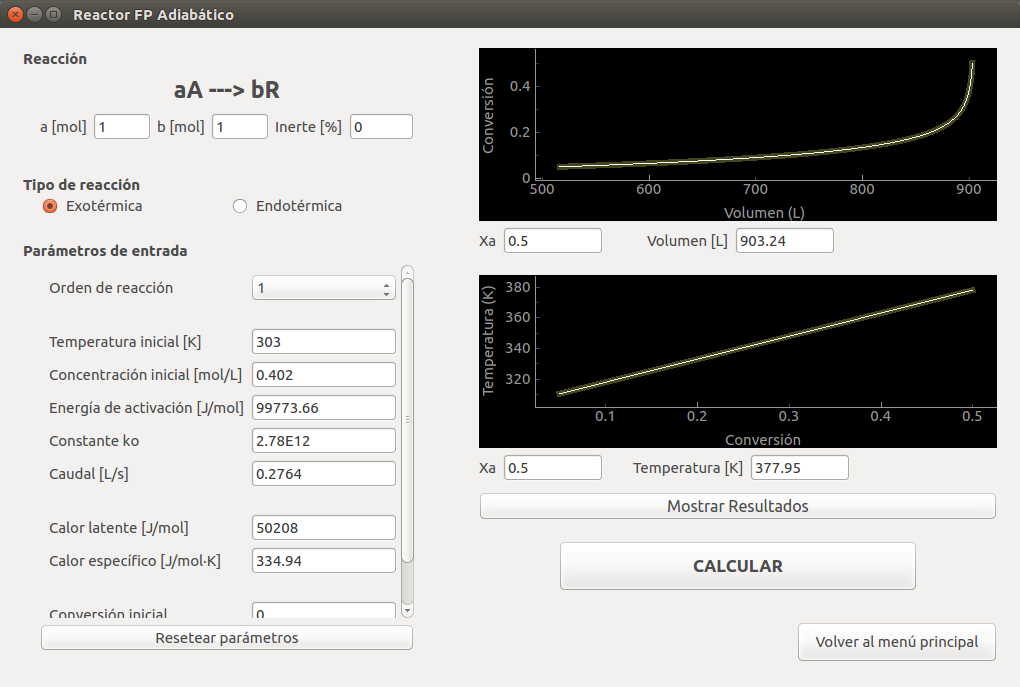
\includegraphics[width=0.85\textwidth]{./imagenes/reactor_fp/adiabatico1.png}\caption{Ventana reactor FP adiabático}\label{fig:ventana_adiabatico}
	\end{center}
\end{figure}

De nuevo, en la parte superior izquierda se nos indica el tipo de reacción con la que vamos a trabajar y permite modificar el número de reactivos y productos, así como añadir el porcentaje deseado de inerte en la reacción. Seguidamente, debido a que estamos trabajando con el caso adiabático, debemos indicar si la reacción será exotérmica o endotérmica. Una vez realizadas estas operaciones, seleccionaremos el orden de reacción en el desplegable y a continuación introduciremos todos los parámetros de entrada indicados, prestando especial atención a las unidades en las que se indican que han de ser introducidos.

Cuando tengamos introducidos todos los datos que se indican, podremos obtener el resultado final pulsado sobre el botón \textbf{'CALCULAR'} situado en la parte derecha de la ventana. Para este reactor, después de pulsar sobre dicho botón, se representarán dos gráficas en lugar de una. Estas gráficas hacen referencia al volumen del reactor (gráfico superior) y a la temperatura de la reacción (gráfico inferior). Los resultados numéricos obtenidos, en función de nuestros parámetros de entrada, se mostrarán en las celdas situadas en la parte inferior de cada uno de los gráficos.

Para ver los resultados en una ventana independiente (Figura \ref{fig:ventana_graficas_ad}) bastará con pulsar sobre el botón \textbf{'Mostrar Resultados'}. En esta nueva ventana, como en el caso anterior, dispondremos de un cursor que nos permitirá movernos a través de ambas curvas para ver el resultado del volumen y la temperatura en cada punto deseado. En esta nueva ventana también se nos permite exportar el gráfico como una imagen.

\begin{figure}[h!]
	\begin{center}
		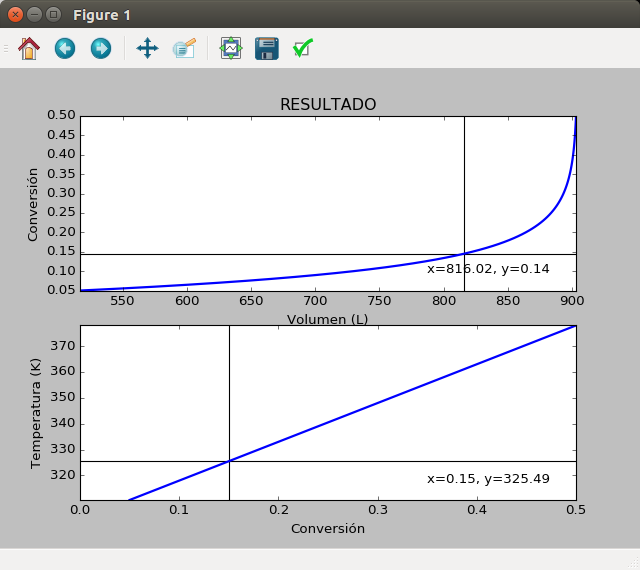
\includegraphics[width=0.85\textwidth]{./imagenes/reactor_fp/adiabatico2.png}\caption{Ventana de resultados reactor FP adiabático}\label{fig:ventana_graficas_ad}
	\end{center}
\end{figure}

Finalmente, podemos realizar un borrado de todas las celdas, mediante el botón \textbf{'Resetear parámetros'}, para realizar un nuevo cálculo. Si no deseamos realizar más cálculos y queremos regresar al menú principal, podremos hacerlo pinchando sobre el botón mediante el botón \textbf{'Volver al menú principal'} de abajo a la derecha de la ventana.


\section{Reactor flujo pistón no adiabático y no isotermo}
Seleccionando el reactor flujo pistón no adiabático y no isotermo, se nos abrirá una ventana como la mostrada en la Figura \ref{fig:ventana_noadi_noiso}.

\begin{figure}[h!]
	\begin{center}
		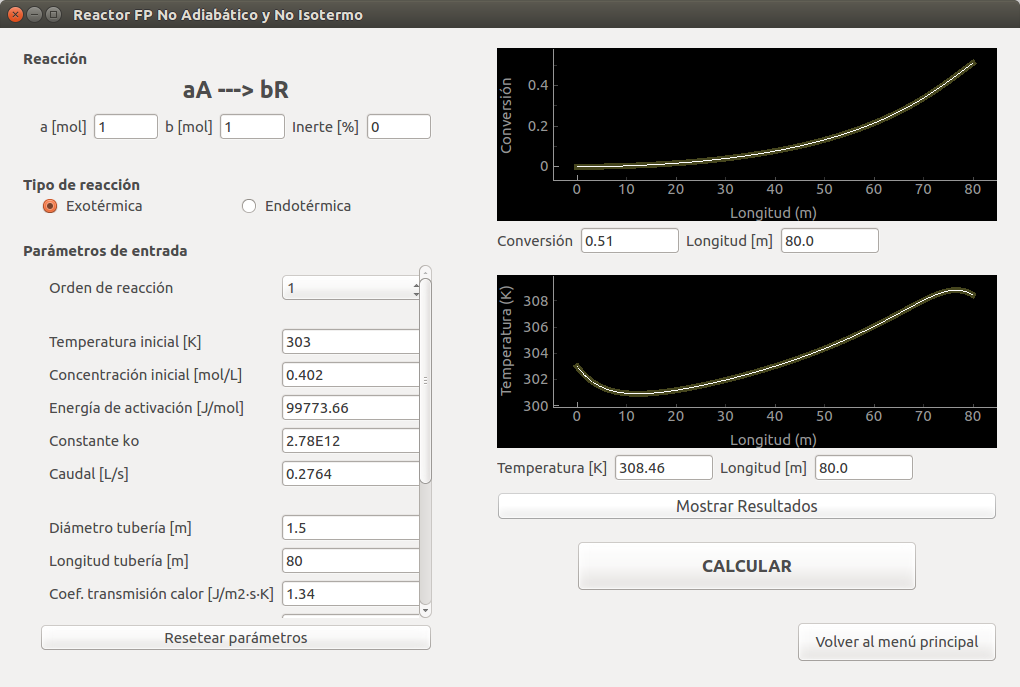
\includegraphics[width=0.85\textwidth]{./imagenes/reactor_fp/no_adi_no_iso1.png}\caption{Ventana reactor FP no adiabático y no isotermo}\label{fig:ventana_noadi_noiso}
	\end{center}
\end{figure}

La estructura de esta venta es similar a la del caso anterior (reactor flujo pistón adiabático), mostrando en la parte superior izquierda el tipo de reacción con la que vamos a trabajar. Permite modificar el número de reactivos y productos, así como añadir el porcentaje deseado de inerte en la reacción. Seguidamente, debemos indicar si la reacción será exotérmica o endotérmica. Una vez realizadas estas operaciones, seleccionaremos el orden de reacción en el desplegable y procederemos a introducir todos los parámetros de entrada indicados, prestando especial atención a las unidades en las que se indican que han de ser introducidos.

Cuando tengamos introducidos todos los datos que se indican, podremos obtener el resultado final pulsado sobre el botón \textbf{'CALCULAR'} situado en la parte derecha de la ventana. Después de pulsar sobre dicho botón, se representarán dos gráficas como ocurría en el caso anterior. Dichas gráficas hacen referencia a la conversión que puede lograr el reactor (gráfico superior) y a la temperatura de la reacción (gráfico inferior), ambas en función de la longitud de la tubería. Los resultados numéricos obtenidos, en función de nuestros parámetros de entrada, se mostrarán en las celdas situadas en la parte inferior de cada uno de los gráficos.

\begin{figure}[h!]
	\begin{center}
		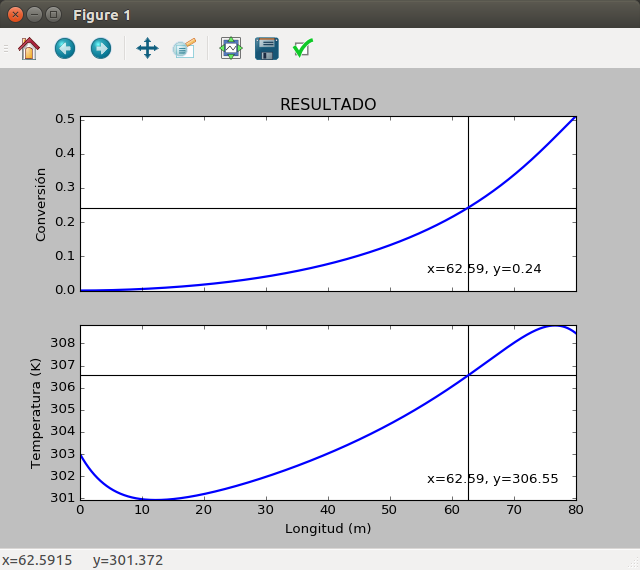
\includegraphics[width=0.85\textwidth]{./imagenes/reactor_fp/no_adi_no_iso2.png}\caption{Ventana de resultados reactor FP no adiabático y no isotermo}\label{fig:ventana_graficas_noadi_noiso}
	\end{center}
\end{figure}

Para ver los resultados en una ventana independiente (Figura \ref{fig:ventana_graficas_noadi_noiso}) bastará con pulsar sobre el botón \textbf{'Mostrar Resultados'}. En esta nueva ventana, como en el caso anterior, dispondremos de un cursor que nos permitirá movernos a través de ambas curvas para ver el resultado de conversión y temperatura en cada punto concreto de la curvas. También podremos exportar el gráfico como una imagen.

Finalmente, podemos realizar un borrado de todas las celdas, mediante el botón \textbf{'Resetear parámetros'}, para realizar un nuevo cálculo. Si no deseamos realizar más cálculos y queremos regresar al menú principal, podremos hacerlo pinchando sobre el botón mediante el botón \textbf{'Volver al menú principal'} de abajo a la derecha de la ventana.
\printindex
\chapter{Reactor Mezcla Perfecta}
En un reactor de mezcla perfecta lo  que  se  consigue  es  que  exista  una  homogeneidad 
perfecta en la reacción, es decir, que todos los puntos tengan la misma temperatura y presión, 
consiguiendo que toda la mezcla que se extraiga tenga idénticas condiciones a la que 
está en el interior del reactor.
	
	En el menú principal, encontramos dos botones dentro del apartado de reactores de mezcla perfecta. Estos dos botones serán utilizados indistintamente en función del propósito que tengamos: cálculo del volumen o cálculo de la conversión.
	
\section{Cálculo del volumen}
Si seleccionamos la opción de cálculo de volumen, nos aparece una ventana como la que se puede observar en la Figura \ref{fig:ventana_volumen}.

\begin{figure}[h!]
	\begin{center}
		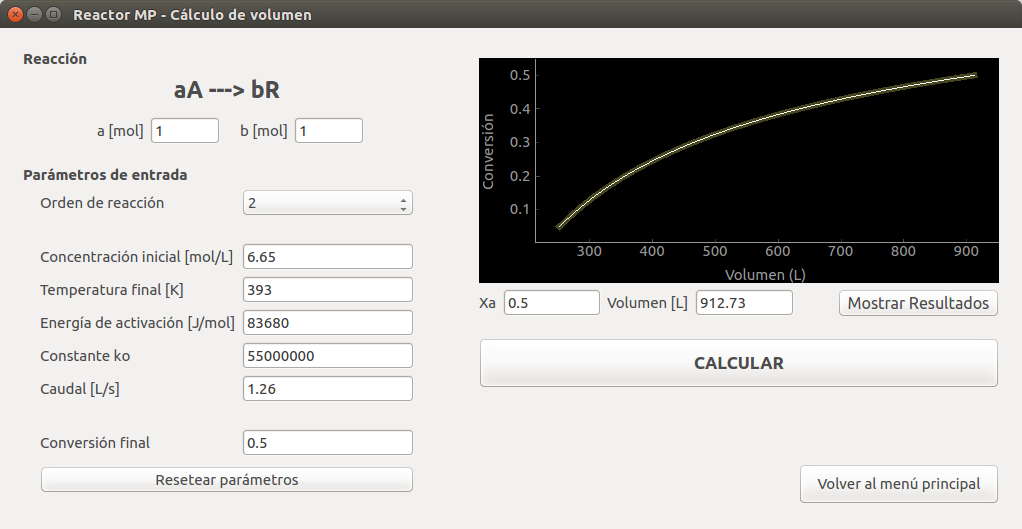
\includegraphics[width=0.85\textwidth]{./imagenes/reactor_fp/mezcla_perfecta1.png}\caption{Ventana reactor MP (cálculo de volumen)}\label{fig:ventana_volumen}
	\end{center}
\end{figure}

En la parte superior izquierda, el programa nos indica el tipo de reacción con la que vamos a trabajar y permite modificar el número de reactivos y productos. Una vez que hayamos establecido la reacción deseada, deberemos seleccionar el orden de reacción en el desplegable e introducir todos los parámetros de entrada indicados, prestando especial atención a las unidades en las que se indican que han de ser introducidos.

Cuando tengamos introducidos todos los datos indicados, podremos obtener el resultado final pulsando sobre el botón \textbf{'CALCULAR'}, situado en la parte derecha de la ventana. Inmediatamente después de pulsar sobre dicho botón el programa representará de forma gráfica el resultado en la parte derecha de la ventana, y se indicará el valor final obtenido como resultado, en función de nuestros parámetros de entrada, en las celdas situadas en la parte inferior del gráfico.

Si deseamos visualizar el gráfico en una ventana independiente ((Figura \ref{fig:ventana_graficas_volumen})), podemos hacerlo pulsado sobre el botón \textbf{'Mostrar Resultados'}. En esta nueva ventana, no solo podremos ver el mismo gráfico descrito anteriormente, sino que además dispondremos de un cursor que nos permitirá ver el resultado en cada punto de la curva. En esta nueva ventana también se nos permite exportar el gráfico como una imagen.

\begin{figure}[h!]
	\begin{center}
		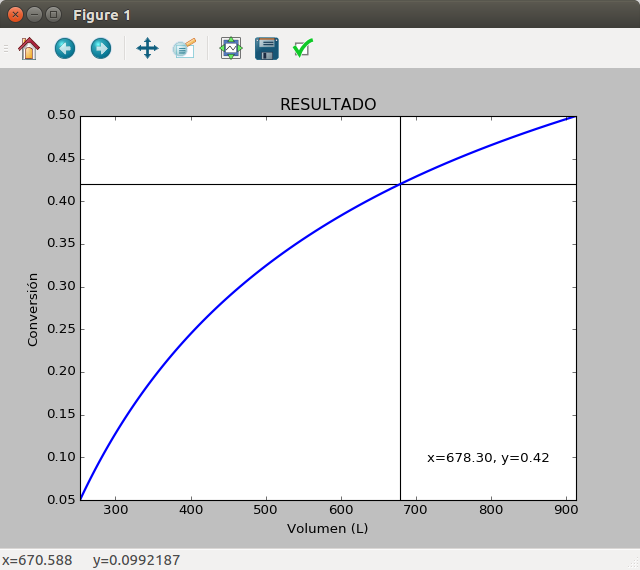
\includegraphics[width=0.85\textwidth]{./imagenes/reactor_fp/mezcla_perfecta2.png}\caption{Ventana de resultados reactor MP (cálculo de volumen)}\label{fig:ventana_graficas_volumen}
	\end{center}
\end{figure}

Finalmente, podemos realizar un borrado de todas las celdas, mediante el botón \textbf{'Resetear parámetros'}, para realizar un nuevo cálculo. Si no deseamos realizar más cálculos y queremos regresar al menú principal, podremos hacerlo pinchando sobre el botón \textbf{'Volver al menú principal'} de abajo a la derecha de la ventana.


\section{Cálculo de la conversión}
Si seleccionamos la opción de cálculo de la conversión, nos aparece una ventana como la que se puede observar en la Figura \ref{fig:ventana_conversion}.

\begin{figure}[h!]
	\begin{center}
		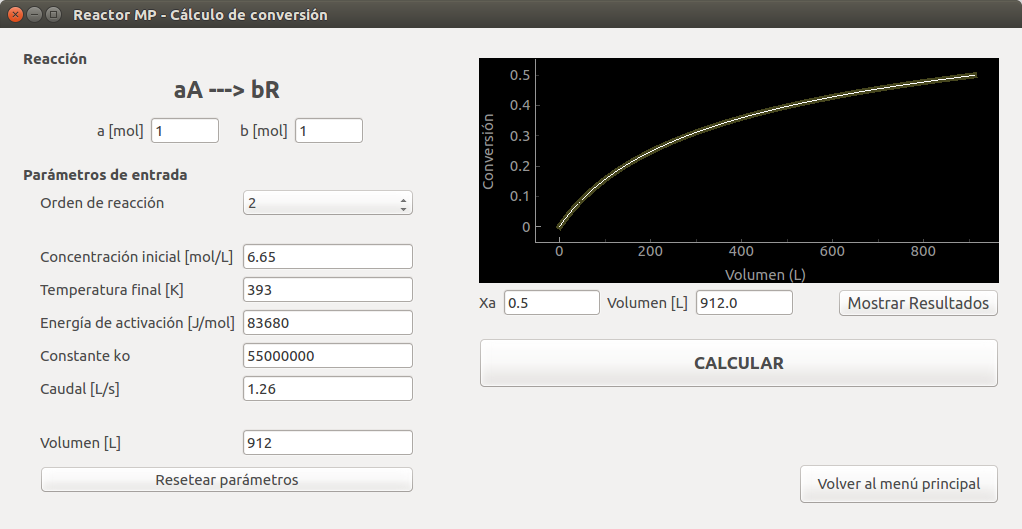
\includegraphics[width=0.85\textwidth]{./imagenes/reactor_fp/mezcla_perfecta3.png}\caption{Ventana reactor MP (cálculo de conversión)}\label{fig:ventana_conversion}
	\end{center}
\end{figure}

Al igual que para el cálculo del volumen descrito anteriormente, se nos informa en la parte superior izquierda de la ventana sobre el tipo de reacción con la que vamos a trabajar y se nos permite modificar el número de reactivos y productos. Una vez realizadas estas operaciones, seleccionaremos el orden de reacción en el desplegable y a continuación introduciremos todos los parámetros de entrada indicados, prestando especial atención a las unidades en las que se indican que han de ser introducidos.

Podremos obtener el resultado final, una vez que hayamos introducido todos los datos, pulsando sobre el botón \textbf{'CALCULAR'} situado en la parte derecha de la ventana. Así se representará el resultado en el gráfico de la parte derecha de la ventana. Además, los resultados numéricos obtenidos como solución final, en función de nuestros parámetros de entrada, se mostrarán en las celdas situadas en la parte inferior del gráfico mencionado.

Si deseamos ver los resultados en una ventana independiente (Figura \ref{fig:ventana_graficas_conversion}) bastará con pulsar sobre el botón \textbf{'Mostrar Resultados'}. En esta nueva ventana, como en el caso anterior, dispondremos de un cursor que nos permitirá movernos a través de la curva obtenida para ver el resultado en cada punto concreto. En esta nueva ventana también se nos permite exportar el gráfico como una imagen.

\begin{figure}[h!]
	\begin{center}
		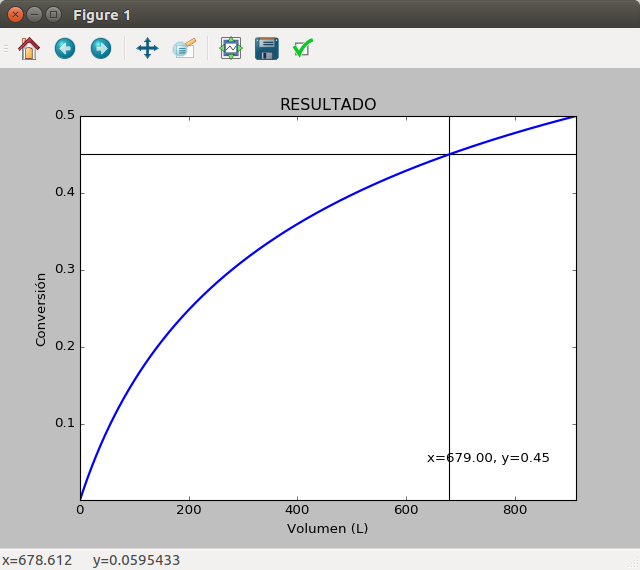
\includegraphics[width=0.85\textwidth]{./imagenes/reactor_fp/mezcla_perfecta4.png}\caption{Ventana de resultados reactor MP (cálculo de conversión)}\label{fig:ventana_graficas_conversion}
	\end{center}
\end{figure}

Finalmente, podemos realizar un borrado de todas las celdas, mediante el botón \textbf{'Resetear parámetros'}, para realizar un nuevo cálculo. Si no deseamos realizar más cálculos y queremos regresar al menú principal, podremos hacerlo mediante el botón \textbf{'Volver al menú principal'}, situado en la parte inferior derecha de la ventana.

\printindex
\end{document}